\documentclass[10pt,a4paper]{article}
\usepackage[utf8]{inputenc}
\usepackage[T1]{fontenc}
\usepackage[brazilian]{babel}
\usepackage{fullpage}
\usepackage{graphicx}
\usepackage{paralist}
\usepackage{multicol}
\usepackage{hyperref}

\hypersetup{
	pdftitle={Poster do Trabalho da disciplina de "Recuperação de Dados pelo Conteúdo"},
	pdfauthor={Arthur F. M. Nascimento}
}

\title{Desenvolvimento de um software de recuperação de imagens por similaridades usando tecnologias FLOSS\cite{FLOSS}}
\author{Arthur Nascimento (tureba@gmail.com)}
\date{Novembro de 2010}

\begin{document}
\begin{titlepage}
\begin{center}
{\Large Desenvolvimento de um software de recuperação de imagens por similaridades usando tecnologias FLOSS\cite{FLOSS}}

\vspace*{0.2cm}

{\Large ICMC - USP - 2º Semestre de 2010}

\vspace*{0.2cm}

{\large Arthur Nascimento (tureba@gmail.com)\\\url{http://github.com/tureba/CBIR}}
\end{center}

\tiny

\begin{multicols}{2}
\section{Introdução}

O objetivo deste trabalho é implementar um sistema de recuperação de imagens
por similaridade de características. O sistema deve poder responder a duas
perguntas previstas: 1) Quais são as N imagens do BD que estão mais próximas
da imagem fornecida? e 2) Quais imagens do BD estão a até uma distância R
da imagem fornecida? Para ambas as perguntas, devem ser usados os vetores
de características extraídos de todas as imagens do BD e da imagem de
referência fornecida na consulta, assim como uma das funções de distância
escolhida no acionamento da busca.

A interface é apresentada na primeira figura:

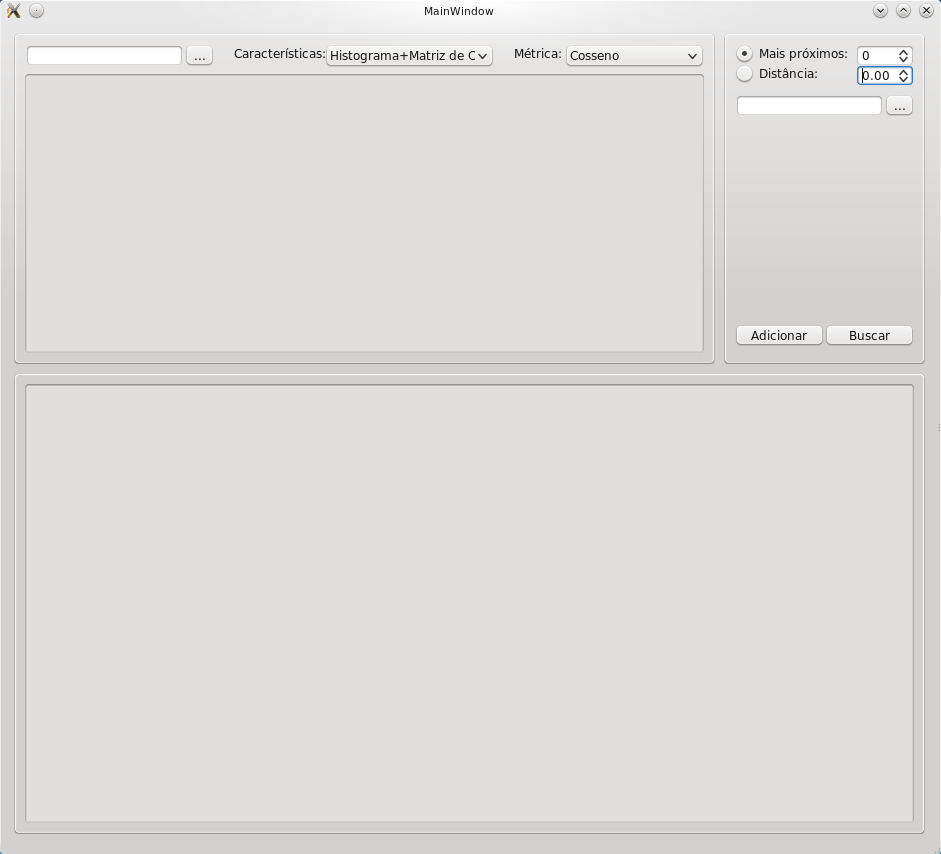
\includegraphics[scale=0.25]{CBIR_inicial.png}


\subsection{Requisitos}

Alguns requisitos mínimos de implementação foram propostos:

\begin{itemize}
	\item Interface com o usuário;
	\item Ao menos 4 funções de distância/similaridade;
	\item Ao menos 2 algoritmos de extração de vetores de características;
	\item E, ou o uso de uma estrutura de dados multidimensional;
	\item Ou a implementação de um algoritmo de realimentação de relevância.
\end{itemize}


\section{Sobre o Software}

O sistema foi desenvolvido em C++ com o auxílio da biblioteca Qt\cite{qt4},
que implementa a interface, e da biblioteca Arboretum\cite{arboretum}, que
fornece uma estrutura de dados multidimensional customizável.

As funções de distância e similaridade implementadas foram:
\begin{itemize}
	\item Distância de Minkowski com parâmetro 2 (Distância Euclidiana);
	\item Distância Irakura-Saito;
	\item Divergência de Kullback-Leibler;
	\item Dissimilaridade dos Cossenos.
\end{itemize}

As funções de extração de características implementadas até o momento:
\begin{itemize}
	\item Histograma;
	\item Matriz de Co-Ocorrência com uma distância (1 pixel) e quatro
		ângulos (0, 45, 90 e 135).
\end{itemize}

Entre o uso de uma estrutura de dados muldidimensional e a implementação de
um algoritmo de realimentação de relevância foi escolhida a primeira opção
através do uso da biblioteca Arboretum\cite{arboretum}, desenvolvida pelo GBDI/ICMC/USP,
que pode ser obtida de \url{http://www.gbdi.icmc.usp.br/old/arboretum/} (ou uma versão
com correções minhas em \url{http://github.com/tureba/arboretum}).

A figura seguinte mostra o software com a base de dados de imagens carregada:

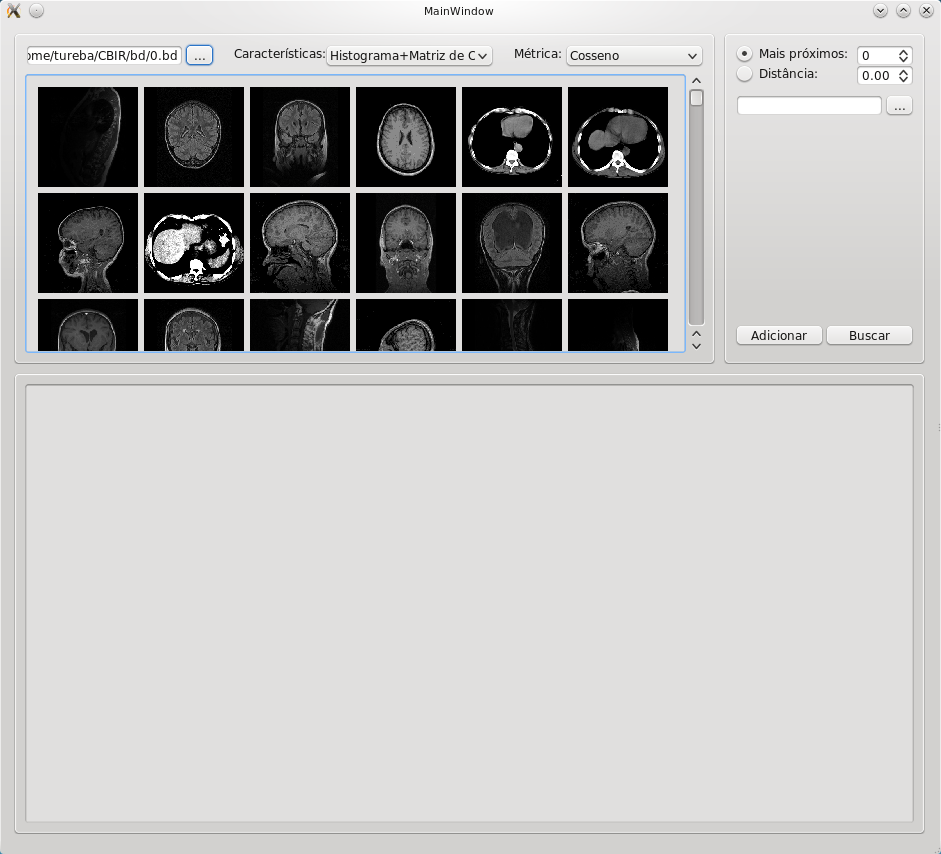
\includegraphics[scale=0.25]{CBIR_bd.png}

A figura seguinte mostra o software com uma imagem antes da consulta ser feita:

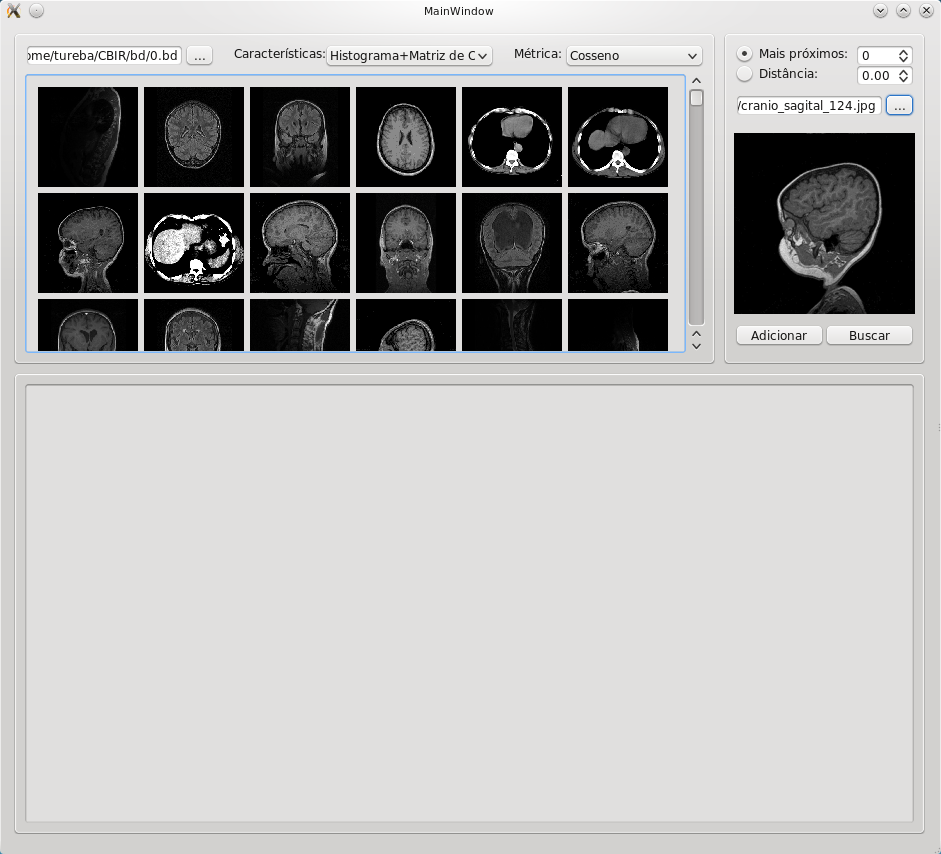
\includegraphics[scale=0.25]{CBIR_imagem.png}


\section{Conclusão}

Através do uso de tecnologias FLOSS\cite{FLOSS}, assim como padrões definidos pela
indústria e pela comunidade, foi possível implementar um software que não só é eficiente,
como também é portável a todas as plataformas que seguem os mesmos padrões. Este
sistema foi desenvolvido em um sistema Exherbo Linux\cite{exherbo} que segue os padrões
POSIX:2008\cite{posix08}, LSB v4.0\cite{lsb4}, FHS v2.3\cite{fhs23}. Esta distribuição Linux
também fornece suporte, através do compilador GCC 4.4\cite{gcc4}, ao próximo padrão da
linguagem C++ conhecido como C++0x\cite{cpp0x}, que foi vital para este software. A biblioteca
Qt\cite{qt4}, por meio da sua flexibilidade também permite que a interface seja exibida corretamente
e com a interatividade esperada em qualquer sistema que a suporte, incluindo todos os derivados de
UNIX e Windows.

Por todas as razões descritas, é visível que as tecnologias FLOSS são uma vantagem para o
desenvolvimento de softwares tanto acadêmicos quando da indústria e tanto protótipos quanto
para produção.

\begin{thebibliography}{99}

	\bibitem{FLOSS} Free/Livre/Open Source Software. \url{http://freeopensourcesoftware.org/}.
	\bibitem{arboretum} Arboretum 2.0. \url{http://www.gbdi.icmc.usp.br/old/arboretum/}.
	\bibitem{qt4} Qt 4.6. \url{http://qt.nokia.com/}.
	\bibitem{gcc4} GCC 4.4. \url{http://gcc.gnu.org/}.
	\bibitem{exherbo} Exherbo Linux. \url{http://www.exherbo.org/}.
        \bibitem{posix08} POSIX:2008. \url{http://www.opengroup.org/onlinepubs/9699919799/}.
	\bibitem{lsb4} LSB v4.0. \url{http://refspecs.freestandards.org/lsb.shtml}.
	\bibitem{fhs23} FHS v2.3. \url{http://www.pathname.com/fhs/}.
	\bibitem{cpp0x} C++0x, The C++ Standards Commitee. \url{http://www.open-std.org/jtc1/sc22/wg21/}.

\end{thebibliography}
\end{multicols}
\end{titlepage}
\end{document}
